\documentclass{beamer}
\usetheme{Dresden} % My favorite!
\usecolortheme{beaver} % Simple and clean template
\usepackage{amssymb,latexsym}
\usepackage{xltxtra, xgreek}

\setsansfont[Mapping=tex-text]{CMU Concrete}
\setmonofont{Courier New}

%\usetheme{Boadilla} % Pretty neat, soft color.
%\usetheme{default}
%\usetheme{Warsaw}
%\usetheme{Bergen} % This template has nagivation on the left
%\usetheme{Frankfurt} % Similar to the default 
%with an extra region at the top.
%\usecolortheme{seahorse} % Simple and clean template
%\usetheme{Darmstadt} % not so good
% Uncomment the following line if you want %
% page numbers and using Warsaw theme%
% \setbeamertemplate{footline}[page number]
\setbeamercovered{transparent}
%\setbeamercovered{invisible}
% To remove the navigation symbols from 
% the bottom of slides%
\setbeamertemplate{navigation symbols}{} 
%
\usepackage{graphicx}
%\usepackage{bm}         % For typesetting bold math (not \mathbold)
%\logo{\includegraphics[height=0.6cm]{yourlogo.eps}}
%
\title[Elliptic Curve Cryptography]{Υλοποίηση αταλλαγής κλειδιού DH και ψηφιακών υπογραφών βασισμένη σε ελλειπτικές καμπύλες}
\author{Νίκος Γιανναράκης\\ \and Ζωή Παρασκευοπούλου}

\institute[]
{
Σχολή Ηλεκτρολόγων Μήχανικών και Μηχανικών Υπολογιστών\\
Εθνικό Μετσόβιο Πολυτεχνείο
}
\date{\today}

\begin{document}

\begin{frame}
\titlepage
\end{frame}
%$y^2 = x^3 + a \cdot x + b \; , \; x,y,a,b \in \mathcal{R}$
\begin{frame}
\frametitle{Κρυπτογραφία με ελλειπτικές καμπύλες}
\begin{block}
{Why elliptic curve cryptography?}
\begin{itemize}
\item Αυξημένη ασφάλεια με μικρότερα μεγέθη κλειδιών
\item Μειωμένο υπολογιστικό κόστος
\item Ιδανικές για φορητές συσκευές (κινητά κλπ.)
\end{itemize}
\end{block}
\end{frame}
%
\begin{frame}
\frametitle{Ελλειπτικές καμπύλες στο $\mathcal{R}$}
\begin{block}
{Ορισμός}
Μία ελλειπτική καμπύλη στο $\mathcal{R}$ μπορεί να οριστεί ως το σύνολο των σημείων (x,y) που ικανοποιούν μία εξίσωση ελλειπτικής καμπύλης της μορφής: 
$$y^2 = x^3 + a \cdot x + b \; , \; x,y,a,b \in \mathcal{R}$$
μαζί με ένα σημείο $\mathcal{O}$, το οποίο ονομάζουμε σημείο στο άπειρο.
\end{block}
\begin{block}
{Ορισμός πράξεων}
\begin{itemize}
\item Πρόσθεση δύο σημείων $P,Q$
\item Διπλασιασμός ενός σημείου $P$
\end{itemize}
\end{block}
\end{frame}

%
\begin{frame}
\frametitle{Πρόσθεση δύο σημείων πάνω σε ελλειπτικές καμπύλες στο $\mathcal{R}$}
H πρόσθεση δύο σημείων $P, Q$ μπορεί να οριστεί γεωμετρικά
\begin{center}
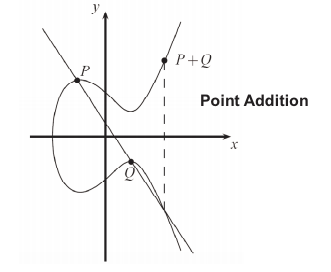
\includegraphics[scale=0.5]{add.png}

\end{center}\end{frame}

%
\begin{frame}
\frametitle{Διπλασιασμός σημείου πάνω σε ελλειπτικές καμπύλες στο $\mathcal{R}$}
Ο διπλασιασμός ενός σημείου πάνω σε μία ελλειπτική καμπύλη ορίζεται γεωμετρικά σύμφωνα με το παρακάτω σχήμα
\begin{center}
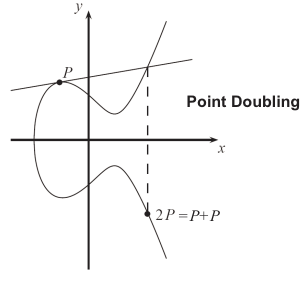
\includegraphics[scale=0.5]{double.png}

\end{center}\end{frame}

%
\begin{frame}
\begin{block}
{Προβλήματα}
\begin{itemize}
\item Αργές πράξεις σε πραγματικούς αριθμούς
\item Έλλειψη ακρίβειας
\end{itemize}
\end{block}
\end{frame}

%
\begin{frame}
\frametitle{Ελλειπτικές καμπύλες πάνω από το $\mathbb{F}_p$ και το $\mathbb{F}_{2^m}$}
\begin{block}
{Ορισμός}
Διαλέγοντας $a,b \in \mathbb{F}_p$  και υπολογίζοντας τα σημεία $(x,y)$ της καμπύλης $modulo \; p$ ορίζουμε μία ελλειπτική καμπύλη στο $\mathbb{F}_p$.
\end{block}
\end{frame}

%
\begin{frame}
\frametitle{Πρόσθεση δύο σημείων πάνω σε ελλειπτικές καμπύλες στο $\mathbb{F}_p$}
H πρόσθεση δύο σημείων $R = P + Q$ σε μία ελλειπτική καμπύλη στο $\mathbb{F}_p$ ορίζεται αλγεβρικά:
 \begin{align*}
 & s = \frac{(y_P - y_Q)}{(x_P - x_Q)}  \pmod p \\
 & x_R = s^2 - x_P - x_Q \pmod p \\
 & y_R = -y_P + s \cdot (x_P - x_R) \pmod p
 \end{align*}
\end{frame}

%
\begin{frame}
\frametitle{Διπλασιασμός σημείου πάνω σε ελλειπτικές καμπύλες στο $\mathbb{F}_p$}
Ο διπλασιασμός σημείου $R = 2P$ σε μία ελλειπτική καμπύλη στο $\mathbb{F}_p$ ορίζεται αλγεβρικά:
 \begin{align*}
  & s = \frac{(3 \cdot x^2_P + a)}{2 \cdot y_P} \pmod p \\
  & x_R = s^2 - 2 \cdot x _P \pmod p \\
  & y_R = -y_p + s \cdot (x_P - x_R) \pmod p
 \end{align*}
\end{frame}

%
\begin{frame}
\frametitle{Βαθμωτός πολλαπλασιασμός πάνω σε ελλειπτικές καμπύλες στο $\mathbb{F}_p$}
Με χρήση των παραπάνω πράξεων μπορούμε να ορίσουμε την πράξη του βαθμωτού πολλαπλασιασμού $R = k \cdot P$ όπου $l \in \mathbb{Z}$ και $P$ ένα σημείο ελλειπτικής καμπύλης.
\begin{itemize}
\item Naive $P + P  \ldots + P$
\item Double-and-add (το ανάλογο του επαναλαμβανόμενου τετραγωνισμού)
\item Windowed, Sliding-window, wNAF, Montogomery ladder $\ldots$ %Cite here
\end{itemize}
\end{frame}

%
\begin{frame}[fragile] % Notice the [fragile] option %
\frametitle{Verbatim}
\begin{example}[Putting Verbatim]
\begin{verbatim}
\begin{frame}
\frametitle{Outline}
\begin{block}
{Why Beamer?}
Does anybody need an introduction to Beamer?
I don't think so.
\end{block}
% Extra carriage return causes problem with verbatim %
\end{frame}\end{verbatim} 
\end{example}
\end{frame}
 
\begin{frame}[fragile]  % notice the fragile option, since the body
			% contains a verbatim command
Example of the \verb|\cite| command to give a reference is below:
Example of citation using \cite{key1} follows on.
\end{frame}
 
\begin{frame}
\frametitle{References}
\footnotesize{
\begin{thebibliography}{99}
 \bibitem[Label1, 2010]{key1} Author's name (1987)
 \newblock Title of the paper.
 \newblock \emph{Journal Name} 55(4), 765 -- 799.
\end{thebibliography}
}
\end{frame}
 
\begin{frame}
\centerline{The End}
\end{frame}
% End of slides
\end{document} 